\subsubsection{Введение}

Продолжая разработку данного программного продукта стало ясно что, несмотря на выбранный шаблон проектирования, добавление нового функционала осложняется тем, что при добавлении новой функции приходится пересобирать весь проект. Это неправльиный подход, так как не позволяет обновлять приложение. Для исправления этой ситуации необходимо доработать архитектуру приложения таким образом, что бы добавление новых функций не приводило к пересборке всего проекта. Это так же позволит проще обновлять проект в дальнейшем. 

После доработки архитектуры, необходимо будет переделать проект, переделать реализацию всего фукционала, а так же свести все ветки разработки в одну, так как на данный момент не все изменения применены к проекту. 

Сформулируем задачи на семестр:

\subsubsection{Задачи на семестр}

\begin{enumerate}
\item переработать архитектуру проекта для более легкого добавления новых функций
\item реализовать данную архитектуру
\item переделать готовые task'и для работы с текущей архитектурой
\item смерджить ветки разработки git
\end{enumerate}

\subsubsection{Новая архитектура}

С увеличением количества тасков возникла проблема с обновлением кода, так как используемый подход предполагал монолитную программу и все таски хоть и были стандартизированы при помощи шаблона разработки factory, всё равно являлись частью основной программы и для добавления тасков или их обновления необходимо постоянно перекомпилировать весь проект. Данная ситуация крайне неудобна при разработки и тестировании, поэтому необходимо было разделить проект на независимые модули.

В языке программирования C++ есть возможность создания библиотек. Библиотеки -- это бинарные файлы в которых хранится коллекции классов и функций. Эти классы и функции можно использовать в любой программе в которой данная библиотека подулючается. Подключать библиотеки в программу можно статически (на этапе компиляции программы) или динамически (непосредственно при выполнении программы). У нашего проекта есть <<скелет>> и таски, каждый из которых работает независимо друг от друга и обменивается данными только со скелетом. 

Так как каждая библиотека является самостоятельным файлом с исполняемым кодом, то для его создания и изменения необходим отдельный проект разработки, а значит если мы захотим изменить что-либо внутри библиотеки, то практически наверняка нам не нужно будет перекомпилировать весь проект. Это значительно упрощает операцию обновления программного комплекса. Было принято решение вынести реализацию всех функций скелета в отдельную статическую библиотеку. А все таски оформить в виде динамических библиотек. 

Данное решение повлекло за собой ряд проблем:
\begin{enumerate}
\item Необходимо разработать структуру динамических библотек для тасков программного комплекса;
\item Необходимо изменить механизм работы с тасками;
\item Необходимо изменить механизм разбора и передачи параметров в основной части программного комплекса;
\item Разработать механизм передачи информации в механизм разбора и передачи параметров.
\end{enumerate}

\subsubsection{библиотеки в С++ и их использование}

Библиотеки предоставляют программисту возможность использовать при разработке программы готовые фрагменты кода. В библиотеки могут быть включены подпрограммы, структуры данных, классы, макросы. В QT для создания библиотеки необходимо укахать в pro-файле проекта добавить строчку \\
TEMPLATE = lib\\
Данная строчка указывает компилятору на то, что мы компилируем библиотеку. После чего в файле исходного кода описывается всё необходимое и после компиляции мы получим файл библиотеки. Для создания динамической библиотеки необходимо добавить в pro-файл ещё строчку: \\
CONFIG += dll\\
А так же в заголовочном файле библиотеки поместить описание прототипов функций которые мы хотим подключать динамически в конструкцию\\
extern <<C>>{ <<описание прототипов>> }\\
Это необходимо для того, что бы при сборке библиотеки функции не поменяли имена. Если не добавить данную конструкцию, то компилятор при сборке изменит имена функций и обратиться к ним динамически не получится.

Для использования разработанной статической библиотеки необходимо просто указать в файле исходного кода строчку \\
\# include <<abolute/part/to/library/file>> \\
Либо поместить созданную библиотеку в папку с системными библиотеками (или добавить в настройки операционной системы путь до созданной библиотеки), тогда можно подключать библиотеку так же как и стандартные библиотеки (имя библиотеки в треугольных скобках)

Динамические библиотеки используются по-другому. Загрузка функции из динамической библиотеки происходит в три этапа: 

\begin{enumerate}
\item Загрузка библиотеки;
\item Описание шаблона для вызова функции:
\item Вызов функции.
\end{enumerate}

В качестве примера на рисунке \ref{ris:dinLib} представлен пример вызова функции foо, которая принимает на вход один аргумент типа int и возвращает его удвоенное значение. функция находится в библиотеке exampleLib. Загрузка библиотеки производится при помощи средств, предоставляемых Qt framework: 
%вот тут короче рисуночек dinLib из папки images

\begin{figure}[ht] 
\center{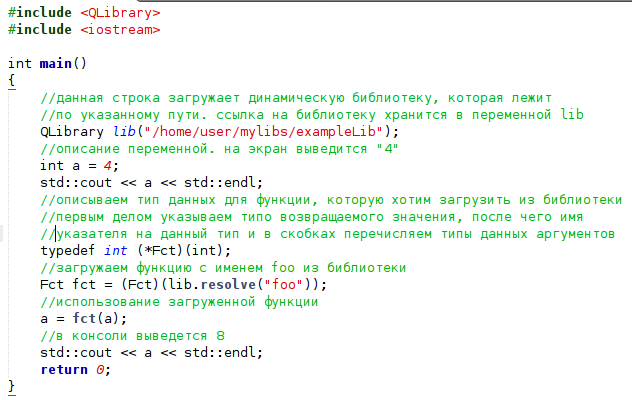
\includegraphics[width=1\linewidth]{dinLib}}
\caption{Пример вызова функции foo}
\label{ris:dinLib}
\end{figure}

\subsubsection{task = динамическая библиотека}

Для того, что бы программа могла работать с каждым таском, как с динамической библиотекой, необходимо что бы все библиотеки были созданы по одному шаблону. То есть в каждой библиотеке должен быть определенный набор функций с определенным именем и входными параметрами к которым можно обращаться при загрузки библиотеки. 

В каждой библиотеке необходимо определить две функции:

\begin{enumerate}
\item функция, возвращающая информацию о таске (имя таска и возможный набор параметров, предназначенных для данного таска)
\item функция выполнения данного таска, которая возвращает логическое значение по окончанию работы, на вход она принимает переменную со всеми настройками, введенными пользователем
\end{enumerate}

На данный момент механизм разбора флагов не был реализван. Структура библиотеки представлена на рисунке \ref{ris:exampleLib}.
%вот тут короче рисунок exampleLib из папки images

\begin{figure}[ht] 
\center{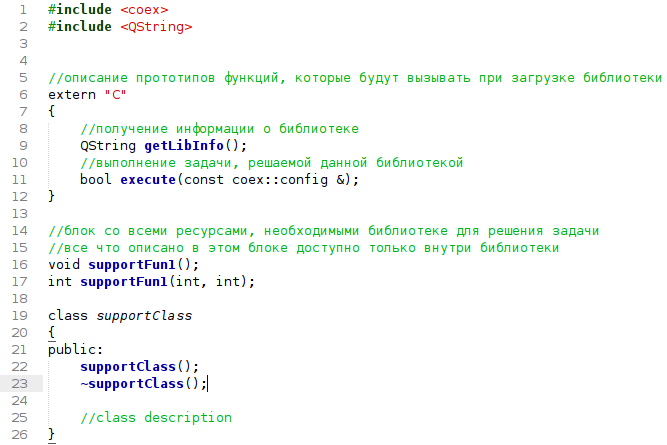
\includegraphics[width=1\linewidth]{exampleLib}}
\caption{Структура библиотеки}
\label{ris:exampleLib}
\end{figure}

Все реализованные таски были оформлены в виде динамических библиотек. Алгоритмы обработки данных изменению не подвергались.

\subsubsection{новый механизм работы с тасками}

Для того, что бы было возмодно добавлять в наш комплекс новые таски без перекомпиляции скелета комплекса мы оформили их в виде динамических библиотек, каждая из которых реализована по шаблону, рассмотренному выше. Все библиотеки, которые мы хотим загружать при работе программы мы помещаем в специальную дирректорию libs рядом с исполняемым файлом. При запуске программа просматривает данную дирректорию и поочередно загружает каждую библиотеку и запускает её на выполнение (если это возможно). 

Алгоритм работы данного механизма представлен на рисунке \ref{ris:initTasks}
%вот тут короче рисунок initTasks из папки images

\begin{figure}[ht] 
\center{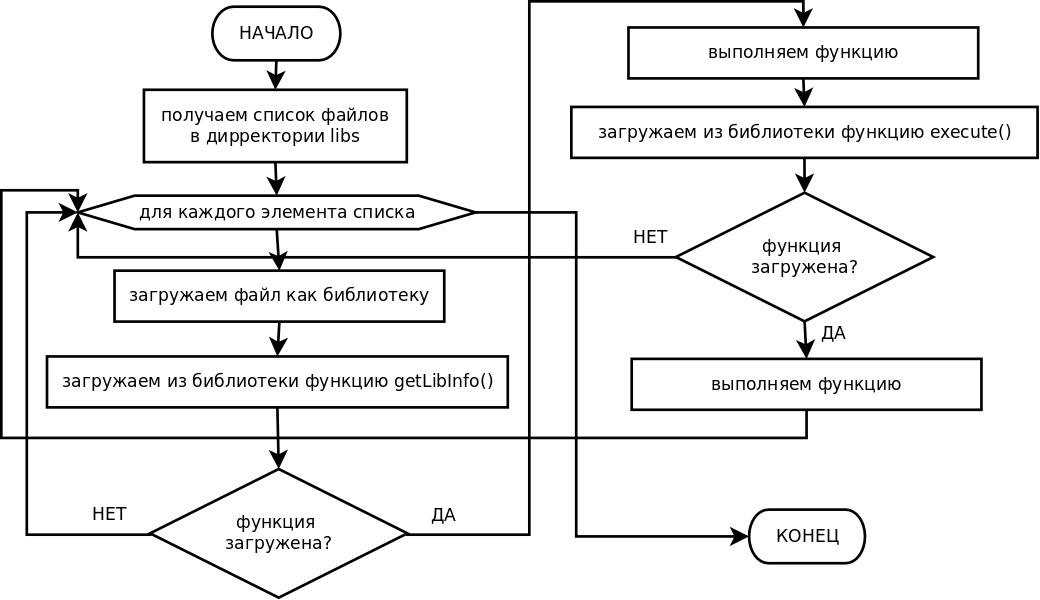
\includegraphics[width=1\linewidth]{initTasks}}
\caption{Пример вызова функции foo}
\label{ris:initTasks}
\end{figure}

\subsubsection{мерджим ветки git}

Разработка комплекса велась двумя разработчиками, каждый из которых работал в своей ветке разработки системы контроля версий git. Необходимо было собрать все изменнеия проекта воедино. Обычно для этого используются инструменты, предстовавляемые самим gitом, но так как в проекте была изменена архитектура (по сути был создан новый проект, который делали их частей старого), то было принято решение просто получить все изменнеия с каждой ветки для каждого проекта и оформить последнии версии тасков в виде динамических библиотек. Данный подход повзолил избежать процедуры разрешения конфликтов. На данный момент новая версия проекта находится в ветке master и содержит все последнии изменения предыдущего проекта. Разработка первой версии комплекса остановлена и, после того как весь код старого проекта будет использован, данная версия комплекса будет удалена.
